\documentclass[10pt]{article} % Font size - 10pt, 11pt or 12pt

\usepackage[hmargin=1.25cm, vmargin=1.5cm]{geometry} % Document margins
\usepackage[usenames,dvipsnames]{xcolor} % Allows the definition of hex colors

\usepackage{listings}
\lstset{escapechar=\&}

% Fonts and tweaks for XeLaTeX
\usepackage{fontspec,xltxtra,xunicode}
\defaultfontfeatures{Mapping=tex-text}
%\setmonofont[Scale=MatchLowercase]{Andale Mono}

% Colors for links, text and headings
\usepackage{hyperref}
\definecolor{linkcolor}{HTML}{506266} % Blue-gray color for links
\definecolor{shade}{HTML}{F5DD9D} % Peach color for the contact information box
\definecolor{text1}{HTML}{2b2b2b} % Main document font color, off-black
\definecolor{headings}{HTML}{701112} % Dark red color for headings
% Other color palettes: shade=B9D7D9 and linkcolor=A40000; shade=D4D7FE and linkcolor=FF0080

\hypersetup{colorlinks,breaklinks, urlcolor=linkcolor, linkcolor=linkcolor} % Set up links and colors

\usepackage{titlesec}
\setcounter{secnumdepth}{4}

\usepackage[utf8]{inputenc}
\usepackage{graphicx}
\usepackage{array}

\setlength{\emergencystretch}{3cm} % somehow helps prevent hboxes from overflowing

\titleformat{\paragraph}
{\normalfont\normalsize\bfseries}{\theparagraph}{1em}{}
\titlespacing*{\paragraph}
{0pt}{3.25ex plus 1ex minus .2ex}{1.5ex plus .2ex}

\usepackage{fancyhdr}
\usepackage{amssymb}
\usepackage{amsmath}
\pagestyle{fancy}
\fancyhf{}

\renewcommand{\headrulewidth}{0pt} % Get rid of the default rule in the header

\bibliographystyle{plain}

\begin{document}

\begin{figure}[h!]
  \centering
  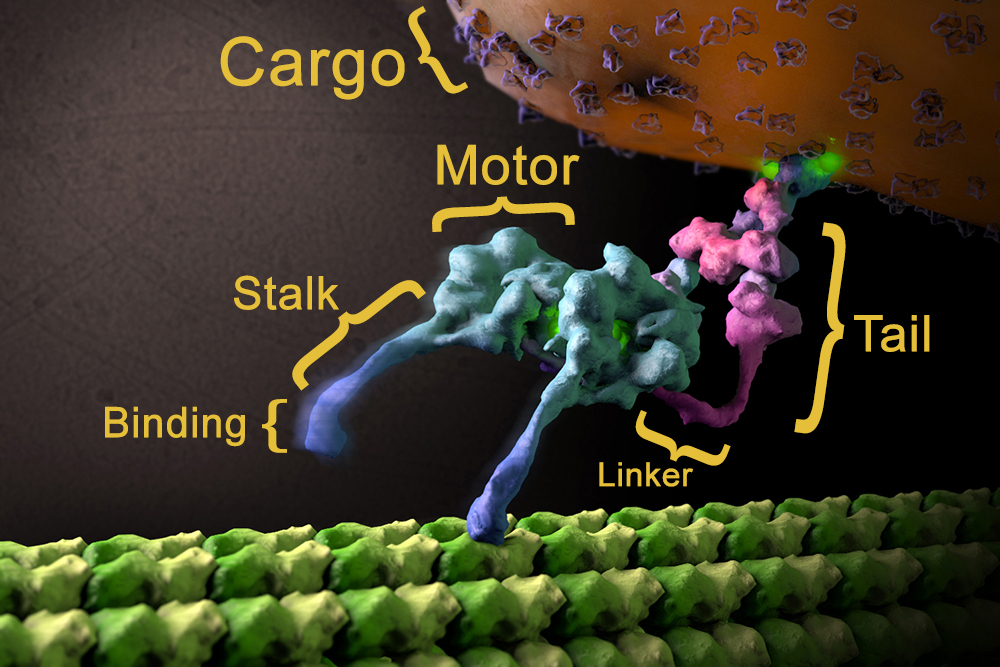
\includegraphics[width=.45\textwidth,keepaspectratio]{../figures/dynein-artist-rendition.jpg}
  \caption{Artist rendition of the dynein motor bound to a microtubule. One monomer is bound to the MT, and one is raised up. Modified. Source: Lander Lab, The Scripps Research Institute.}
  \label{dynein-artist-rendition}
\end{figure}

\begin{figure}[h!]
  \centering
  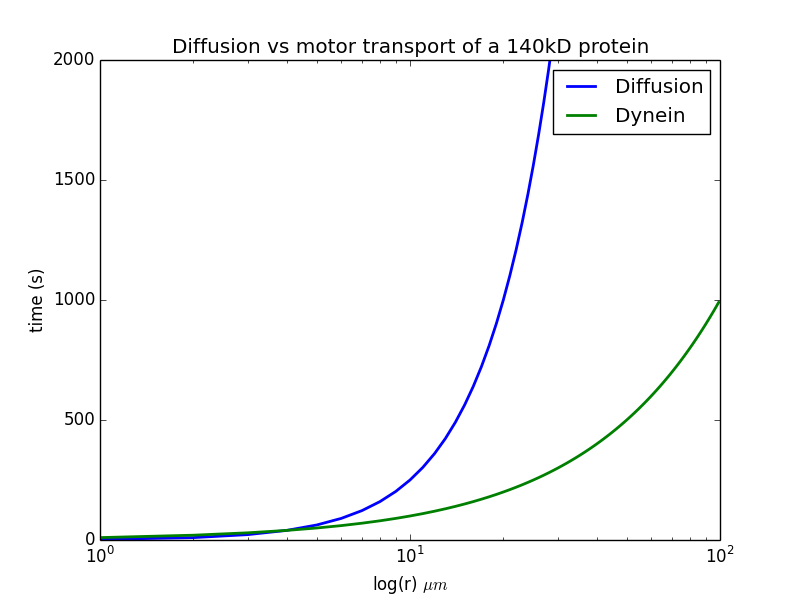
\includegraphics[width=.45\textwidth,keepaspectratio]{../figures/diffusion_vs_dynein.png}
  \caption{Plot comparing the diffusion rate of a 140kD protein with a diffusion consant $D = .2 \mu m^2/s$ with a dynein motor travelling at 100nm/s.}
  \label{diffusion_vs_dynein}
\end{figure}

%% \begin{figure}[h!]
%%   \centering
%%   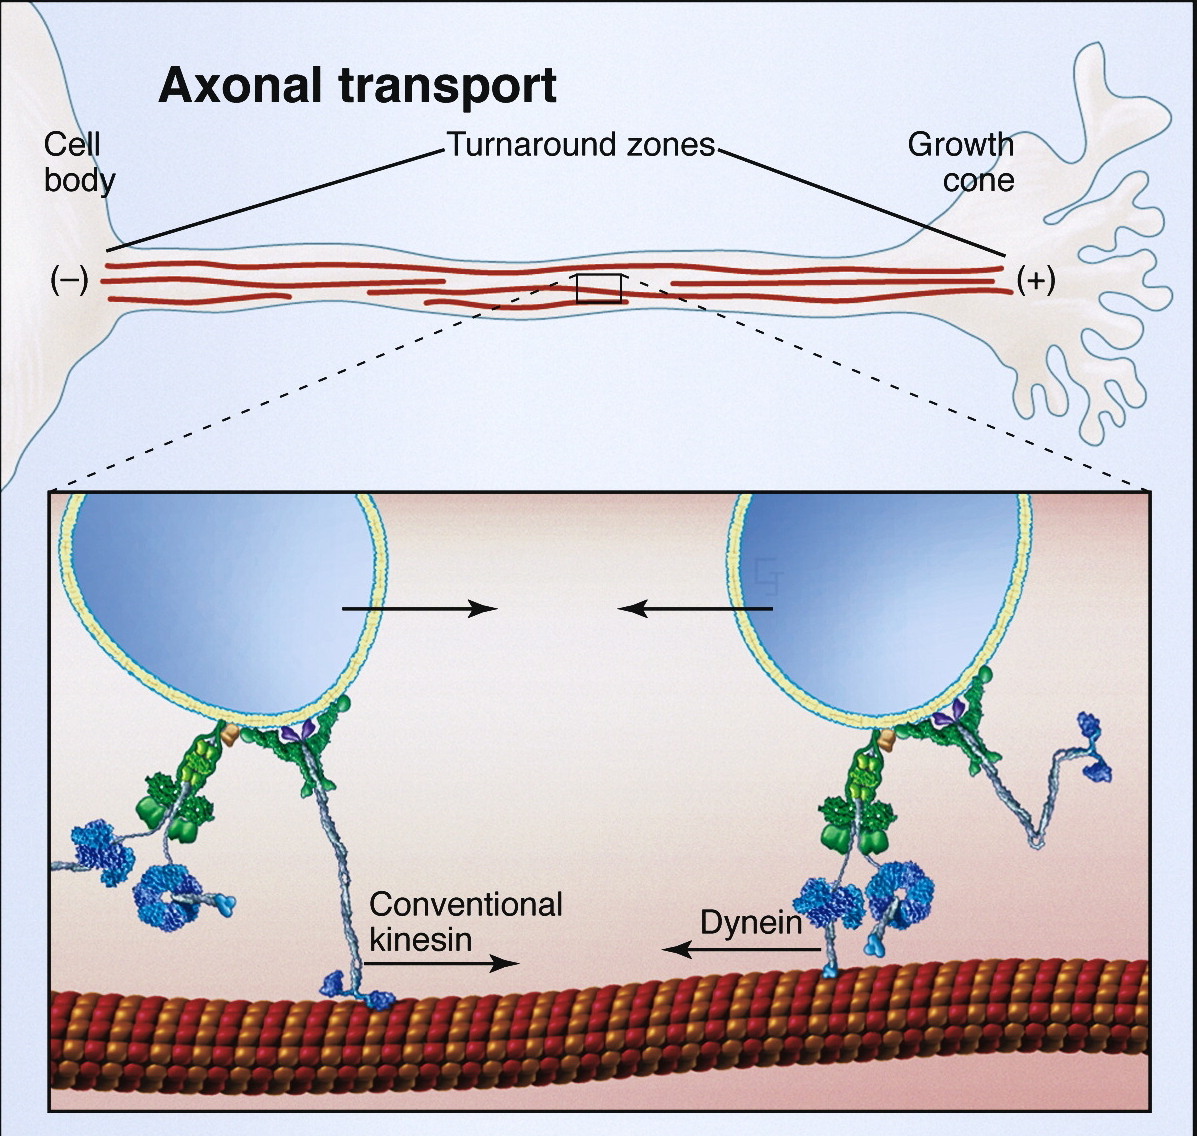
\includegraphics[width=.45\textwidth,keepaspectratio]{../figures/retrograde_transport.jpg}
%%   \caption{Mechanism of dynein localization to axon tips, or growth cones, in retrograde transport mediated by kinesin anterograde transport. Modified from \cite{valetoolbox}.}
%%   \label{retrograde-transport}
%% \end{figure}

%% \begin{figure}[h!]
%%   \centering
%%   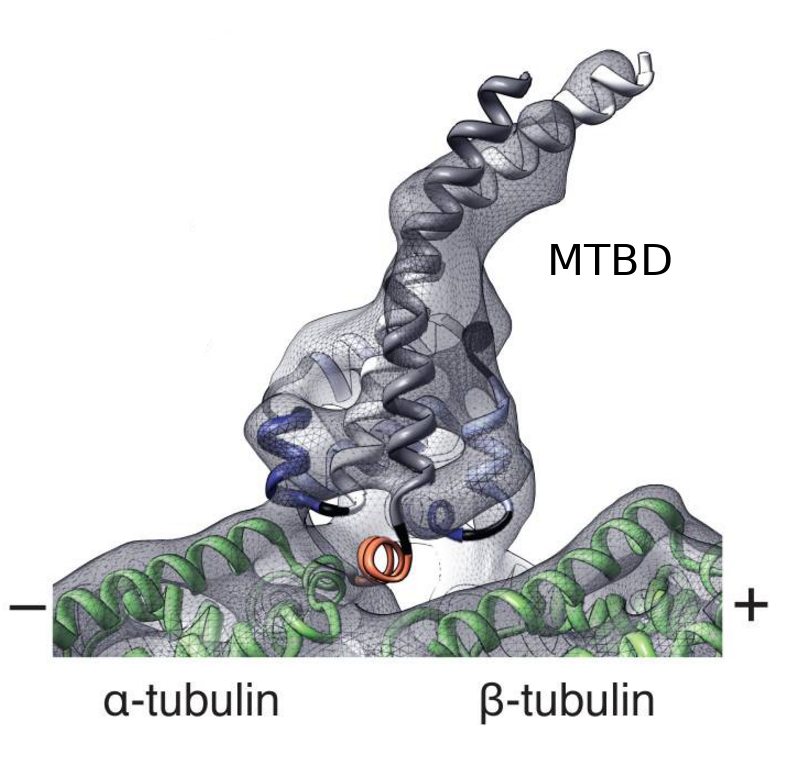
\includegraphics[width=.45\textwidth,keepaspectratio]{../figures/mtbd-complex.png}
%%   \caption{Crystal structure of the MTBD-MT complex. Modified from Redwine \textit{et. al} \cite{redwineMTBDcomplex}.}
%%   \label{dynein-artist-rendition-2}
%% \end{figure}

\begin{figure}[h!]
  \centering
  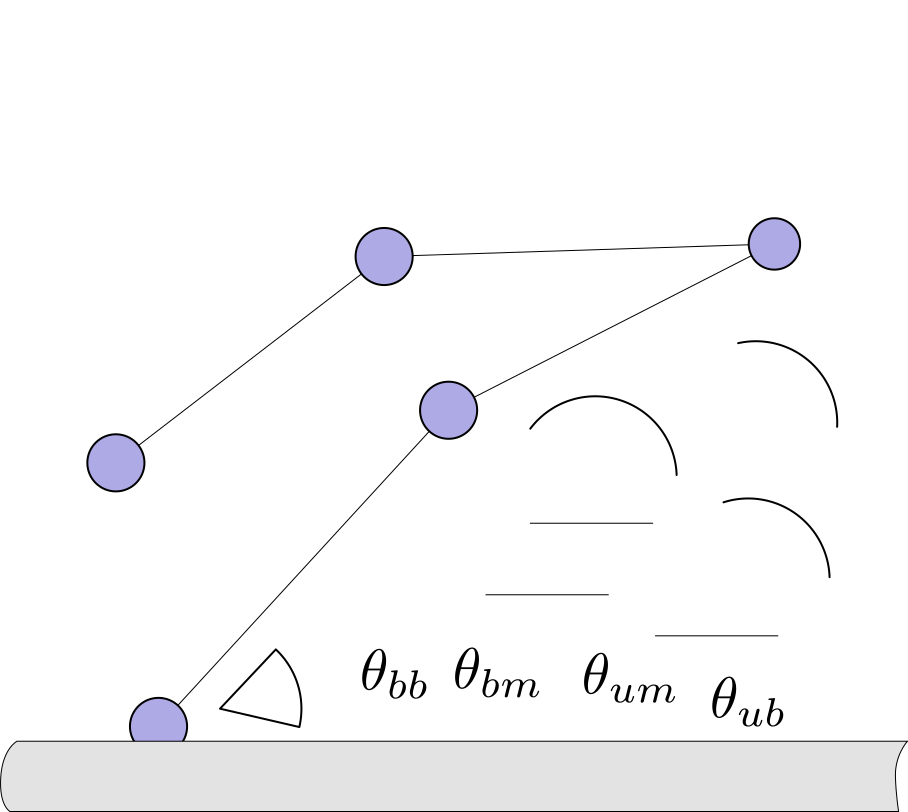
\includegraphics[width=.45\textwidth]{../figures/ob_fig.pdf}
  \caption{Spatial representation of onebound model.}
  \label{ob_fig}
\end{figure}

\begin{figure}[h!]
  \centering
  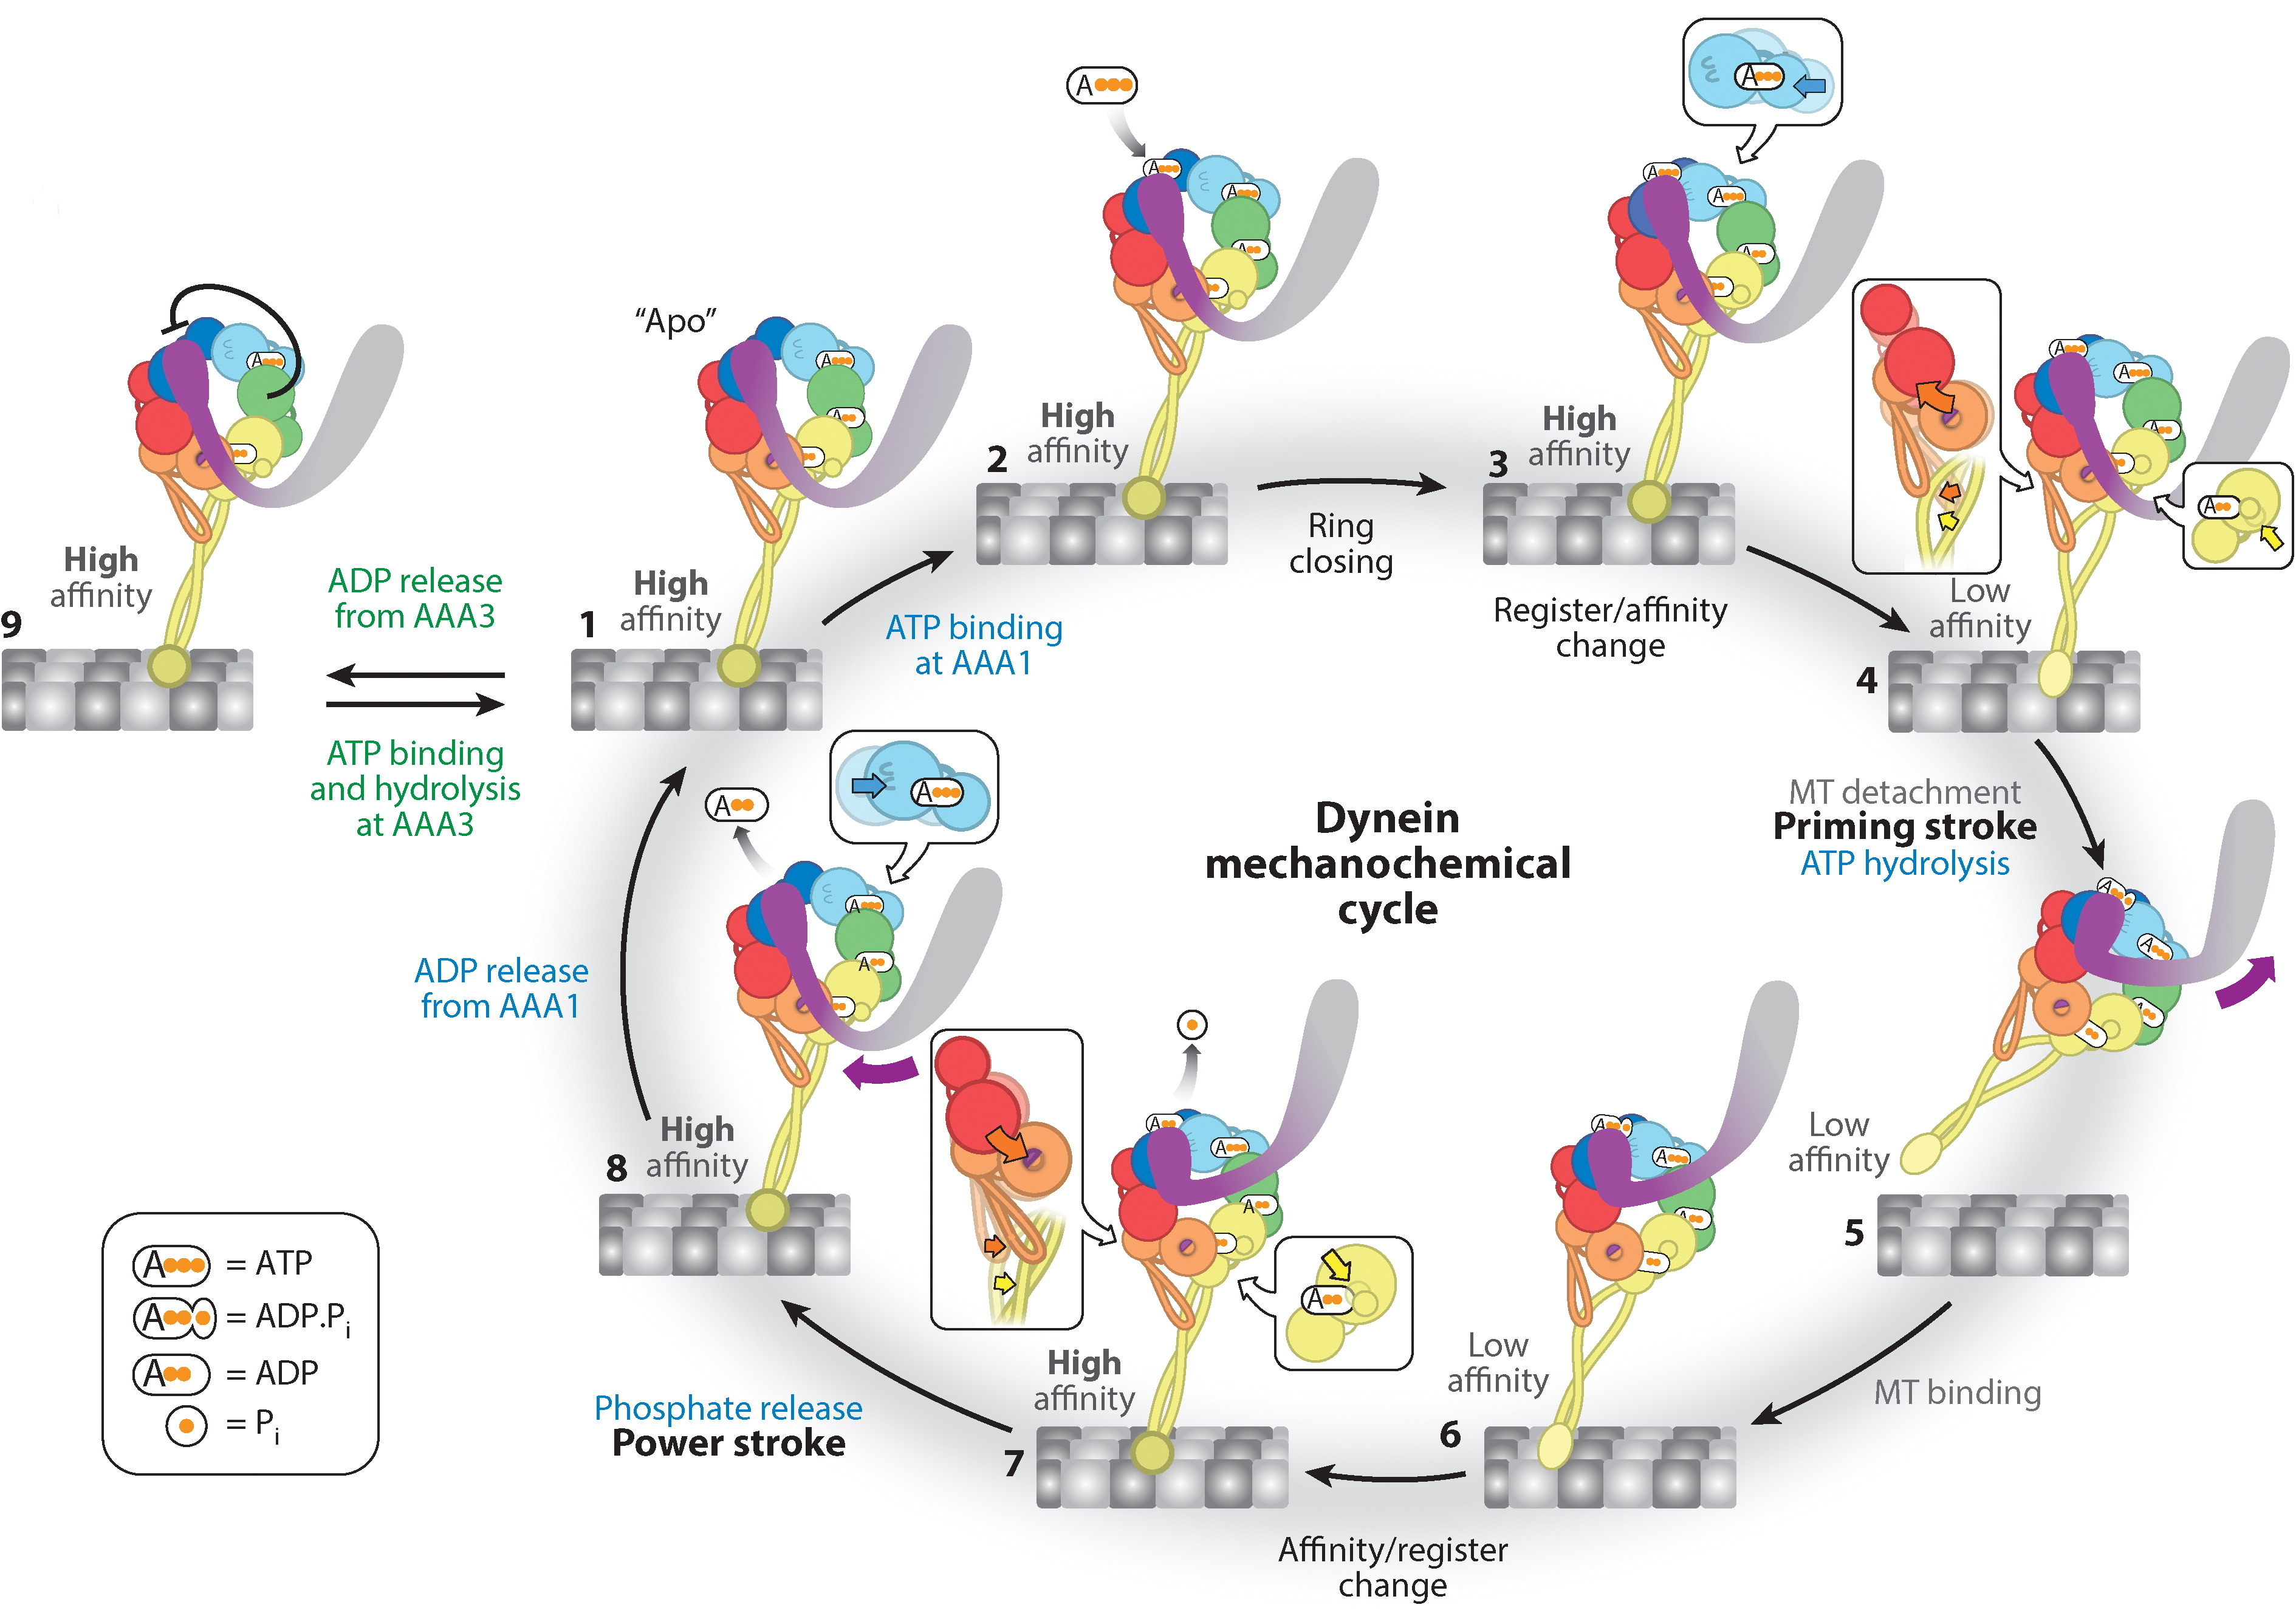
\includegraphics[width=.85\textwidth,keepaspectratio]{../figures/mechanochemical-cycle.jpeg}
  \caption{Cycle of states the dynein motor goes through during motion in the Cianfrocco model \cite{cianfroccoreview}.}
  \label{mech-cycle}
\end{figure}

\begin{figure}[h!]
  \centering
  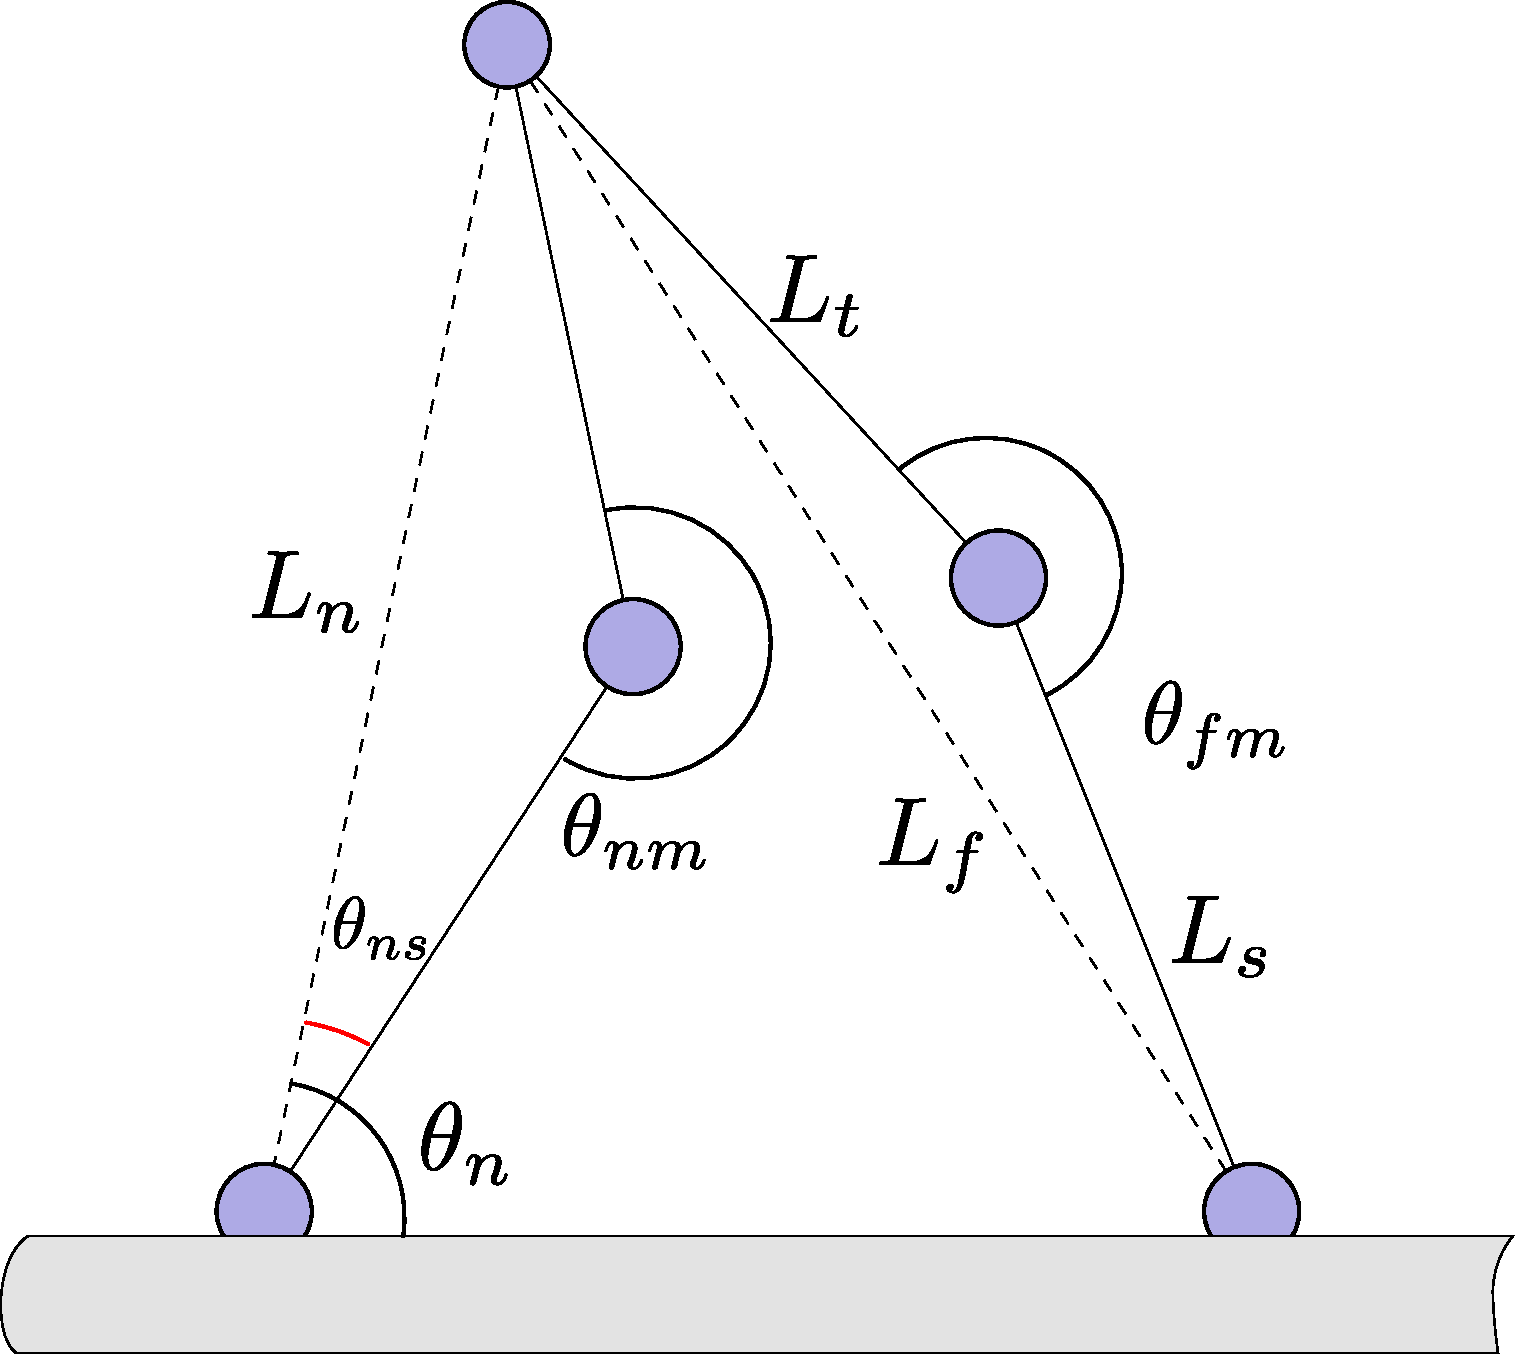
\includegraphics[width=.45\textwidth]{../figures/code-bothbound.pdf}
  \caption{Definition of equilibrium angles.}
  \label{bb_fig}
\end{figure}

\begin{figure}[h!]
  \centering
  \begin{minipage}[b]{0.49\textwidth}
    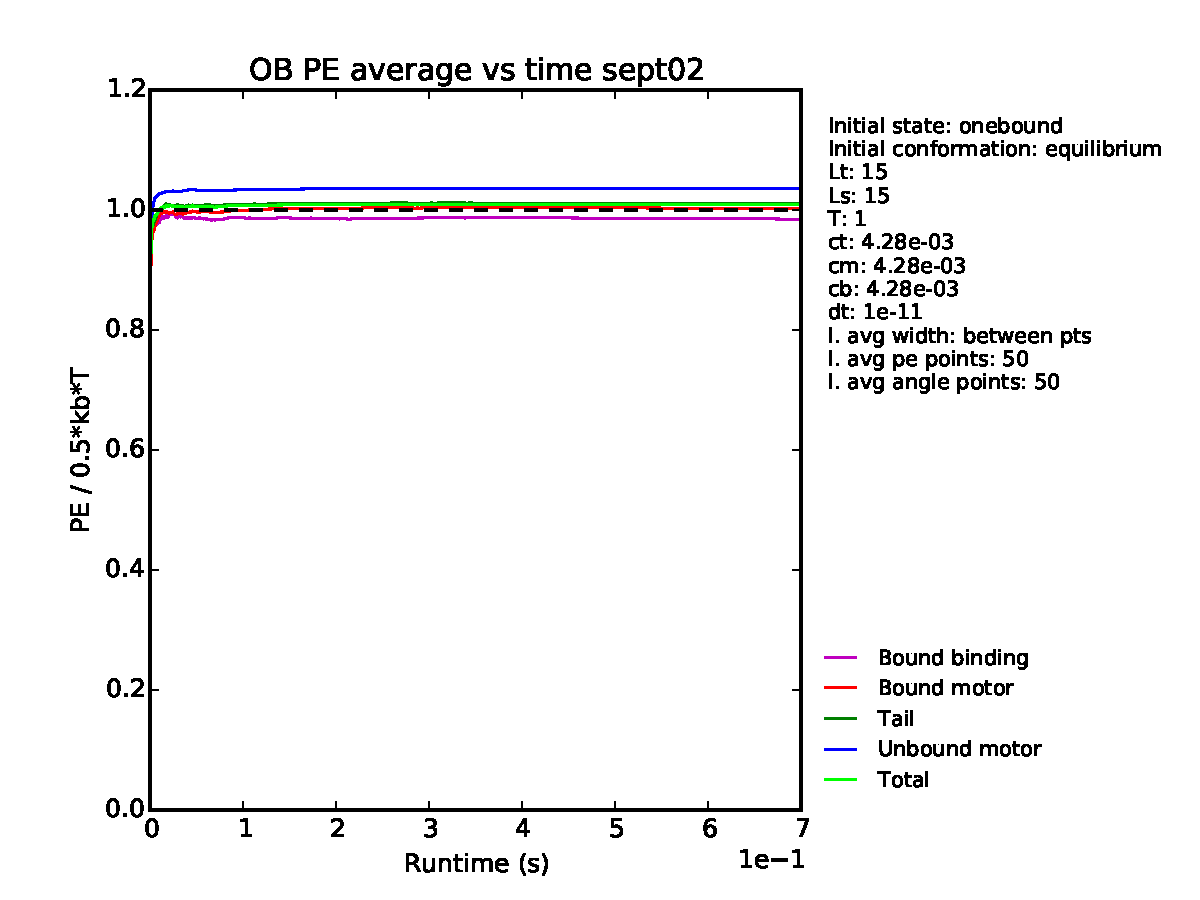
\includegraphics[width=\textwidth]{../figures/OB_Average_PE.pdf}
    \caption{Onebound PE vs time.}
  \end{minipage}
  \begin{minipage}[b]{0.49\textwidth}
    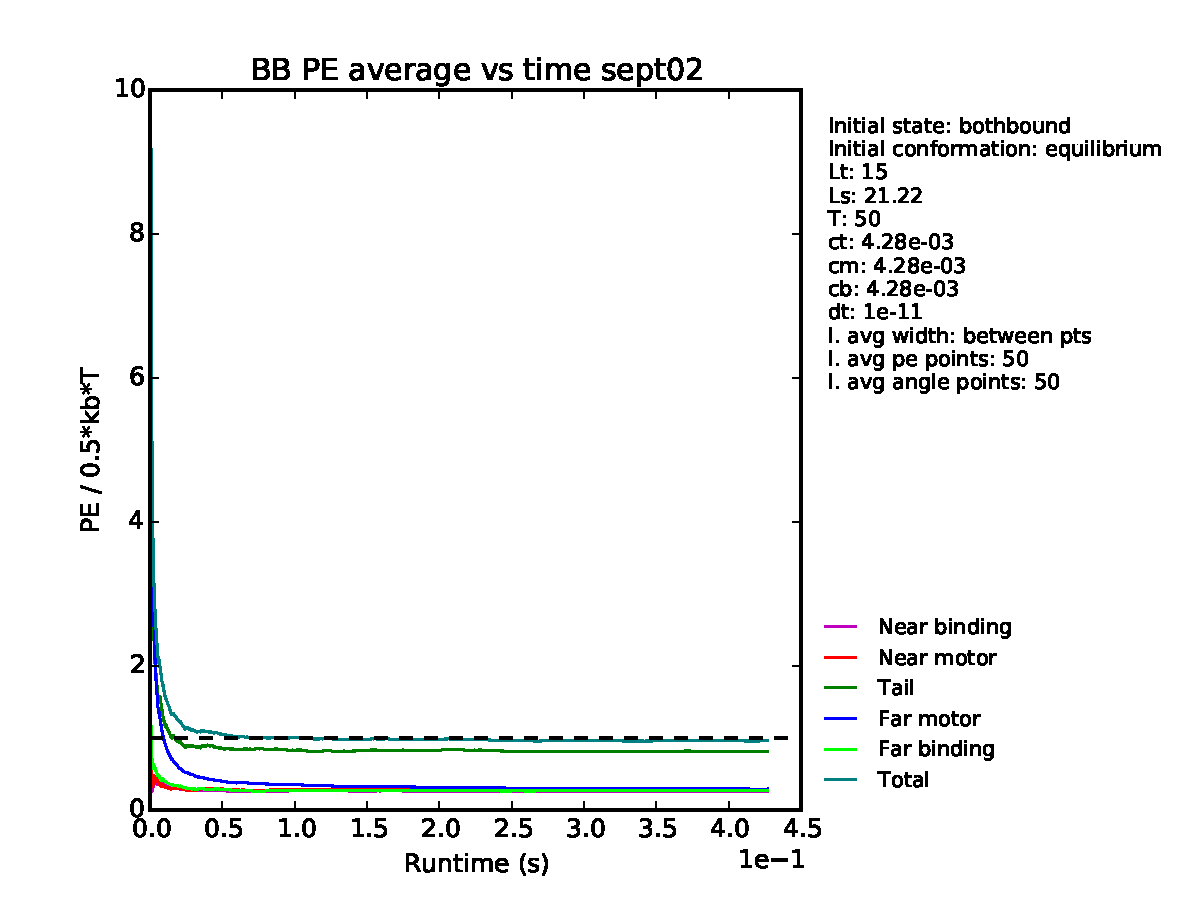
\includegraphics[width=\textwidth]{../figures/BB_Average_PE.pdf}
    \caption{Bothbound PE vs time.}
  \end{minipage}
  \label{equipartition_agreement}
\end{figure}

\begin{figure}[h!]
  \centering
  \begin{minipage}[b]{0.49\textwidth}
    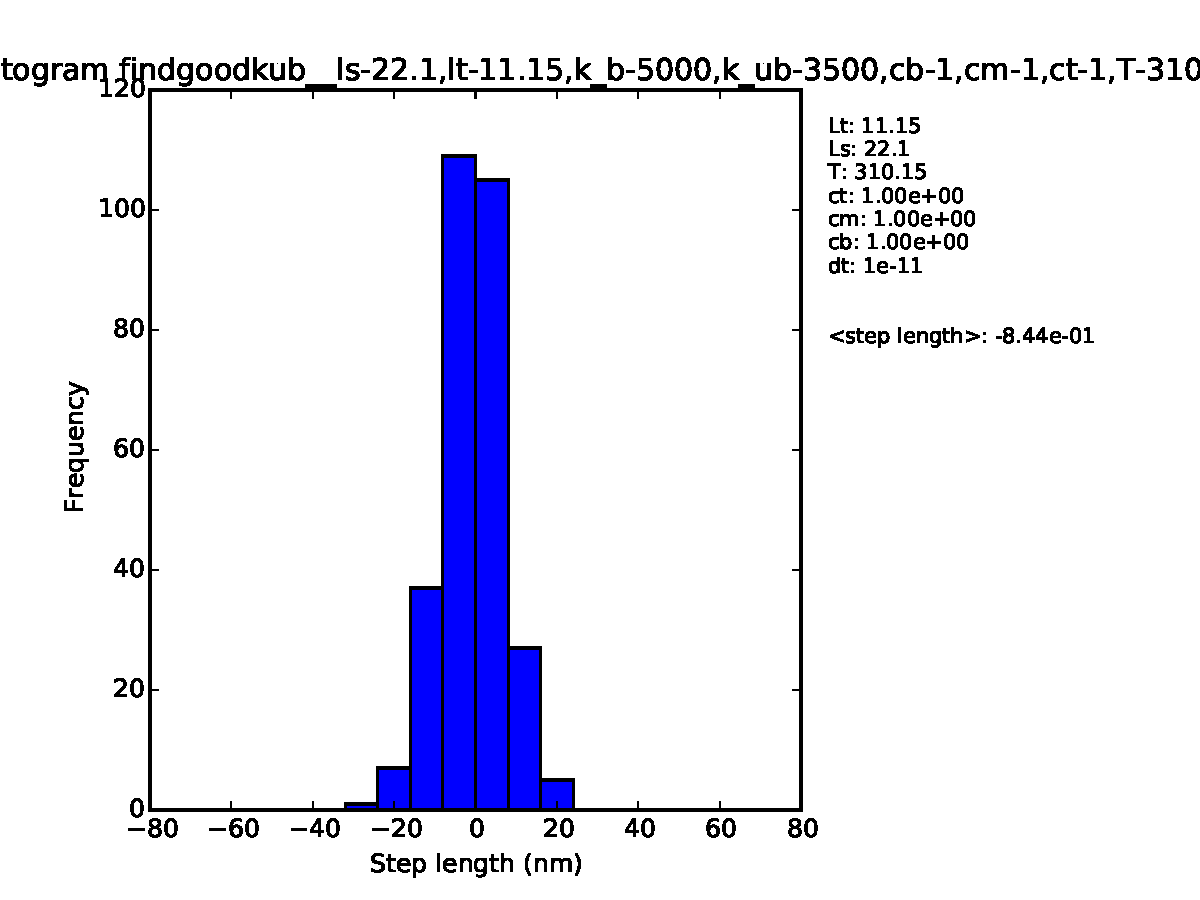
\includegraphics[width=\textwidth]{../figures/length_histogram_sample}
    \caption{Histogram of step lengths over 3 seconds of simulation.}
  \end{minipage}
  \begin{minipage}[b]{0.49\textwidth}
    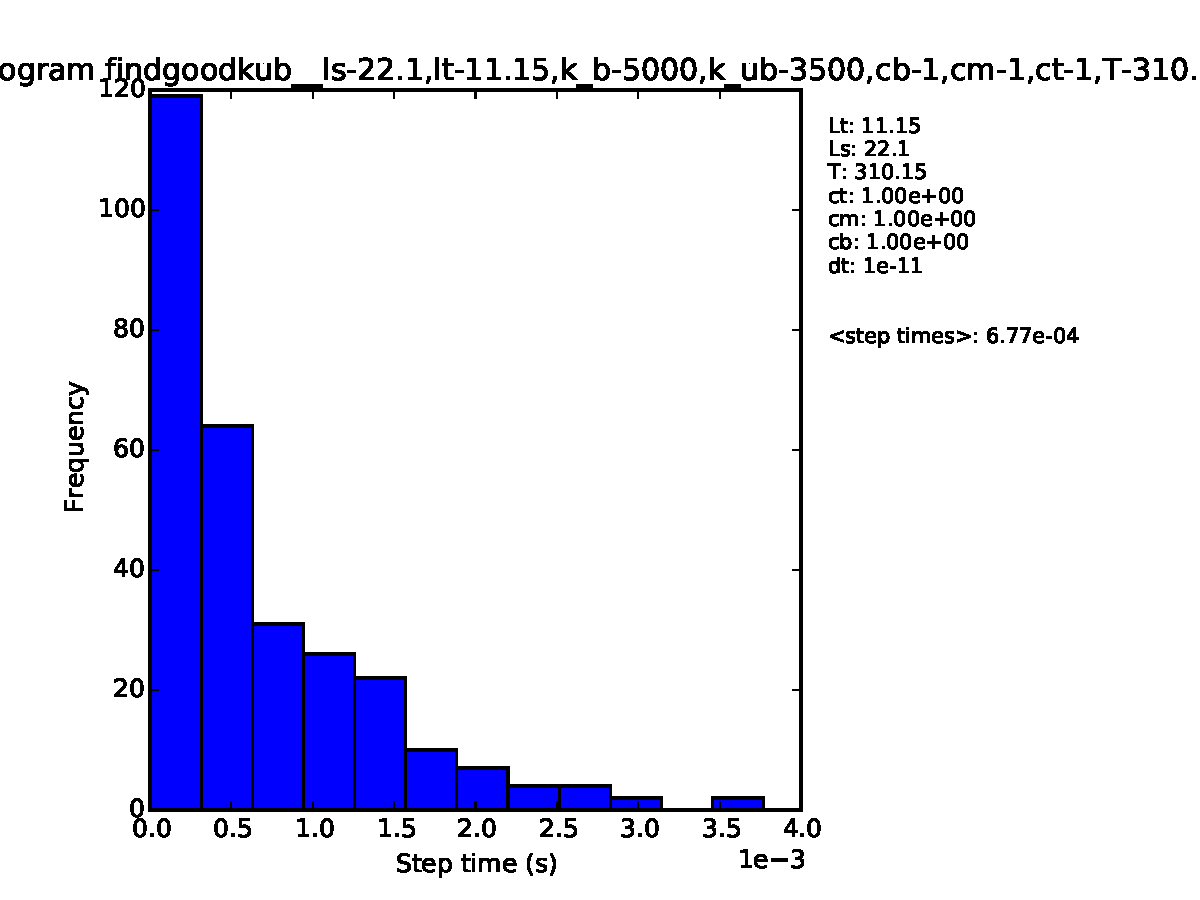
\includegraphics[width=\textwidth]{../figures/time_histogram_sample}
    \caption{Histogram of step times over 3 seconds of simulation.}
  \end{minipage}
\end{figure}

\end{document}
